% !TEX TS-program = xelatex
%
\documentclass[ngerman]{scrartcl}

\usepackage[ngerman]{babel}
\usepackage{amsmath}
\usepackage{enumitem}
\usepackage{graphicx}

\usepackage{siunitx}
\sisetup{per-mode = symbol, binary-units = true}
\DeclareSIUnit\mbyte{Byte}

\usepackage{setspace}% http://ctan.org/pkg/setspace
\usepackage{lipsum}% http://ctan.org/pkg/lipsum
\usepackage{graphicx}
\graphicspath {{assets/}}
\begin{document}

\section*{1}
  \begin{enumerate}[label=\alph*)]
    \item
    \begin{enumerate}[label=\Roman*)]
      \item
      \begin{tabular}{|*{3}{c|}}
        \hline
        $v_i$ & $B_i$ & $O_i$ \\
        \hline
        A & \{B, D\} & \{B\}    \\
        \hline
        B & \{A, D\} & \{A, C\} \\
        \hline
        C & \{B\}    & \{D, E\} \\
        \hline
        D & \{C, E\} & \{A, B\} \\
        \hline
        E & \{C\}    & \{D\}    \\
        \hline
      \end{tabular}
      \begin{doublespacing}
        \begin{tabular}{|l|*{5}{c|}}
          \hline
          Iteration & A & B & C & D & E \\
          \hline
          1 & $\frac{1}{5}$ & $\frac{1}{5}$ & $\frac{1}{5}$ & $\frac{1}{5}$ & $\frac{1}{5}$ \\
          \hline
          2 & $\frac{1}{5}$ & $\frac{3}{10}$ & $\frac{1}{10}$ & $\frac{3}{10}$ & $\frac{1}{10}$ \\
          \hline
          3 & $\frac{3}{10}$ & $\frac{7}{20}$ & $\frac{3}{20}$ & $\frac{3}{20}$ & $\frac{1}{20}$ \\
          \hline
          4 & $\frac{1}{4}$ & $\frac{3}{8}$ & $\frac{7}{40}$ & $\frac{1}{8}$ & $\frac{3}{40}$ \\
          \hline
          5 & $\frac{1}{4}$ & $\frac{5}{16}$ & $\frac{3}{16}$ & $\frac{13}{80}$ & $\frac{7}{80}$ \\
          \hline
          6 & $\frac{19}{80}$ & $\frac{53}{160}$ & $\frac{5}{32}$ & $\frac{29}{160}$ & $\frac{3}{32}$ \\
          \hline
          7 & $\frac{41}{160}$ & $\frac{21}{64}$ & $\frac{53}{320}$ & $\frac{11}{64}$ & $\frac{5}{64}$ \\
          \hline
          8 & $\frac{1}{4}$ & $\frac{219}{640}$ & $\frac{21}{128}$ & $\frac{103}{640}$ & $\frac{53}{640}$ \\
          \hline
        \end{tabular}
      \end{doublespacing}

      \item
      \begin{tabular}{|*{3}{c|}}
        \hline
        $v_i$ & $B_i$ & $O_i$    \\
        \hline
        A & \{E\}     & \{B, C\} \\
        \hline
        B & \{A\}     & \{C\}    \\
        \hline
        C & \{A, B\}  & \{D\}    \\
        \hline
        D & \{C\}     & \{E\}    \\
        \hline
        E & \{D\}     & \{A\}    \\
        \hline
      \end{tabular}
      \begin{doublespacing}
        \begin{tabular}{|l|*{5}{c|}}
          \hline
          Iteration & A & B & C & D & E \\
          \hline
          1 & $\frac{1}{5}$ & $\frac{1}{5}$ & $\frac{1}{5}$ & $\frac{1}{5}$ & $\frac{1}{5}$ \\
          \hline
          2 & $\frac{1}{5}$ & $\frac{1}{10}$ & $\frac{3}{10}$ & $\frac{1}{5}$ & $\frac{1}{5}$ \\
          \hline
          3 & $\frac{1}{5}$ & $\frac{1}{10}$ & $\frac{1}{5}$ & $\frac{3}{10}$ & $\frac{1}{5}$ \\
          \hline
          4 & $\frac{1}{5}$ & $\frac{1}{10}$ & $\frac{1}{5}$ & $\frac{1}{5}$ & $\frac{3}{10}$ \\
          \hline
          5 & $\frac{3}{10}$ & $\frac{1}{10}$ & $\frac{1}{5}$ & $\frac{1}{5}$ & $\frac{1}{5}$ \\
          \hline
          6 & $\frac{1}{5}$ & $\frac{3}{20}$ & $\frac{1}{4}$ & $\frac{1}{5}$ & $\frac{1}{5}$ \\
          \hline
          7 & $\frac{1}{5}$ & $\frac{1}{10}$ & $\frac{1}{4}$ & $\frac{1}{4}$ & $\frac{1}{5}$ \\
          \hline
          8 & $\frac{1}{5}$ & $\frac{1}{10}$ & $\frac{1}{5}$ & $\frac{1}{4}$ & $\frac{1}{4}$ \\
          \hline
        \end{tabular}
      \end{doublespacing}
    \end{enumerate}

    \item
    \resizebox{\textwidth}{!}{
      \begin{doublespacing}
        \begin{tabular}{|l|*{5}{c|}}
          \hline
          Iteration & A & B & C & D & E \\
          \hline
          1 & $\frac{1}{5}$ & $\frac{1}{5}$ & $\frac{1}{5}$ & $\frac{1}{5}$ & $\frac{1}{5}$ \\
          \hline
          2 & $\frac{1}{5}$ & $\frac{27}{100}$ & $\frac{13}{100}$ & $\frac{27}{100}$ & $\frac{13}{100}$ \\
          \hline
          3 & $\frac{249}{1000}$ & $\frac{589}{2000}$ & $\frac{309}{2000}$ & $\frac{393}{2000}$ & $\frac{211}{2000}$ \\
          \hline
          4 & 0.23185 & 0.303075 & 0.163075 & 0.187925 & 0.114075 \\
          \hline
          5 & 0.23185 & 0.28806875 & 0.16607625 & 0.19692875 & 0.11707625 \\
          \hline
          6 & 0.229749125 & 0.2912200625 & 0.1608240625 & 0.2000800625 & 0.1181266875 \\
          \hline
          7 & 0.23195504375 & 0.290852409375 & 0.161927021875 & 0.198977103125 & 0.116288421875 \\
          \hline
          8 & 0.231440329375 & 0.29201051671875 & 0.16179834328125 & 0.19807635296875 & 0.11667445765625 \\
          \hline
        \end{tabular}
      \end{doublespacing}
    }

    \item
    Der Page-Rank, der mit der \texttt{page.rank(g)}-Funktion berechnet wird ist
    immer genau zwischen dem selbst berechneten ohne und mit Dämpfungsfaktor.
    Dass heißt, dass die R-Funktion wahrscheinlich einen Dämpfungsfaktor verwendet,
    der größer als $0,7$ ist.
  \end{enumerate}

\section*{2}
	Festplatte Seagate SkyHawk mit 10tb Speicherkapazität kostet 365€ und wiegt 649g (Daten Amazon)
	\begin{enumerate}[label=\alph*)]
		\item 
		\begin{align*}
			\SI{5,76}{\peta\byte} = \SI{5760}{\tera\byte}
		\end{align*}
		\begin{align*}
			\frac{5760}{10} = 576 \text{ Festplatten}
		\end{align*}
		\begin{align*}
			576 \cdot \SI{649}{\gram} = \SI{373824}{\gram} = \SI{373,824}{\kilogram}
		\end{align*}
		Alle Festplatten passen also in einen LKW.
		
		\item 
		\begin{align*}
			365 \text{€} \cdot 576 = 210240\text{€}
		\end{align*}
				
		\item 
		Die Entfernung von Innsbruck nach Trient beträgt \SI{177}{\kilo\metre}. Bei einer Durchschnittsgeschwindigkeit von \SI{60}{\kilo\metre\per\hour} würde die Fahrt ca \SI{3}{\hour} dauern. 
		\begin{align*}
			\SI{3}{\hour} = \SI{10800}{\second}			
		\end{align*}
		\begin{align*}
			\frac{\SI{5,76}{\peta\byte}}{\SI{10800}{\second}} = \SI{0,5333}{\tera\byte\per\second}		
		\end{align*}
	\end{enumerate}

\section*{3}
	\begin{align*}
		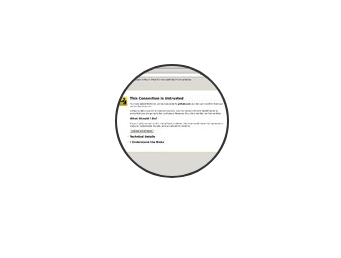
\includegraphics[height=4cm]{assets/github.png}
		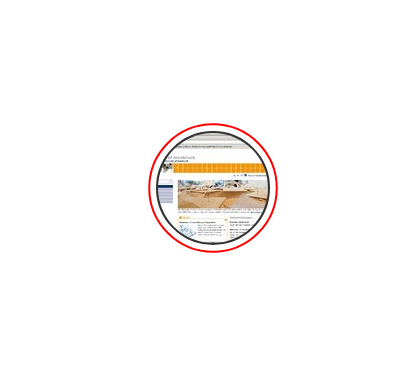
\includegraphics[height=4cm]{assets/uibk.png}
	\end{align*}
	github.com wie auch uibk.ac.at bauen keine weiteren Verbindungen auf. 
	\begin{align*}
		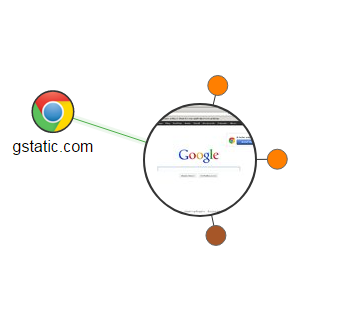
\includegraphics[height=5cm]{assets/google.png}
	\end{align*}
	google.com speichert Cookies welche zur weiteren Verfolgung verwendet werden können.
	\begin{align*}
		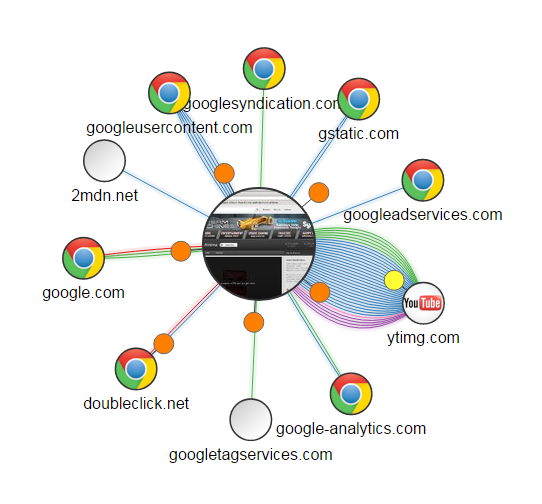
\includegraphics[height=6.5cm]{assets/youtube.png}
	\end{align*}
	youtube.com speichert Cookies und baut Verbindungen zu weiteren google Diensten auf welche zur weiteren Verfolgung verwendet werden können.
	\begin{align*}
		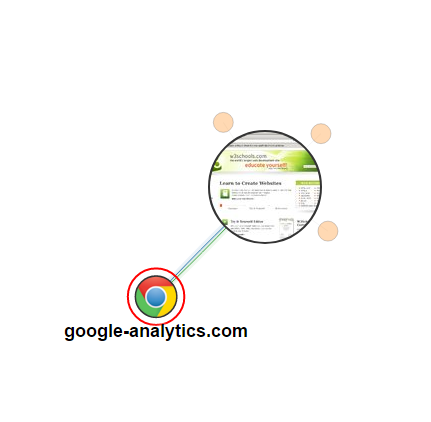
\includegraphics[height=5cm]{assets/w3school.png}
	\end{align*}
	w3school.org speichert Cookies und baut eine Verbindung zu google analytics auf welche zur weiteren Verfolgung verwendet werden können.
	\begin{align*}
		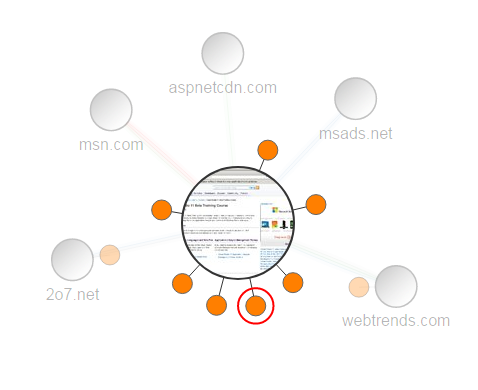
\includegraphics[height=5cm]{assets/msdn.png}
	\end{align*}
	msdn.microsoft.com speichert Cookies und baut Verbindungen zu microsoft Diensten auf.
\section*{5}
  \begin{enumerate}[label=\alph*)]
    \addtocounter{enumi}{1}
    \item
    Eine \texttt{robots.txt}-Datei ist in diesem Fall nutzlos,
    da ein Bot sich nicht an die vorgegebenen Regeln halten muss,
    vor allem nicht einer eines ausländischen Geheimdienstes.
  \end{enumerate}

\pagebreak
\section*{6}
	Zipfsches Gesetz:
	\begin{align*}
		p(n) = \frac{1}{n \cdot \ln(1.78 \cdot n) }
	\end{align*}
	Berechnung:
	\begin{align*}
		p(48) = 1/(48 \cdot \ln(1.78 \cdot 48)) = 0,004683948 \\
		p(47) = 1/(47 \cdot \ln(1.78 \cdot 48)) = 0,004783607 \\
		p(46) = 1/(46 \cdot \ln(1.78 \cdot 48)) = 0,004887598 \\
		p(45) = 1/(45 \cdot \ln(1.78 \cdot 48)) = 0,004996212 \\
		p(44) = 1/(44 \cdot \ln(1.78 \cdot 48)) = 0,005109762 \\
		p(43) = 1/(43 \cdot \ln(1.78 \cdot 48)) = 0,005228594 \\
		p(42) = 1/(42 \cdot \ln(1.78 \cdot 48)) = 0,005353084 \\
		p(41) = 1/(41 \cdot \ln(1.78 \cdot 48)) = 0,005483647 \\
		p(40) = 1/(40 \cdot \ln(1.78 \cdot 48)) = 0,005620738 \\
		p(39) = 1/(39 \cdot \ln(1.78 \cdot 48)) = 0,005764860  \\
		\\
		p(39)+p(40)+p(41)+p(42)+(43)+p(44) \\
		+p(45)+p(46)+p(47)+p(48) = 0,05191205 \\
		\\
		48 - 9 = 39	
	\end{align*}
	Es müssen mindestens 39 Themen gelernt werden um die Prüfung mit einer Wahrscheinlichkeit von 95 \% zu bestehen.


\end{document}
